

%% ------------------- Description of pipeline used in 26-01_27_run2 ----------------------------

%% 1) Input 
The data motivating this project come from a meta-population of Norwegian house sparrows on an island system off the coast of Helgeland. The meta-population spans 18 islands. These islands are divided into two main habitats: the \textit{inner islands}, closer to the mainland, and the \textit{outer islands}, further from the mainland. Some islands are more isolated, but there is genetic flow (dispersal) between all of them (\cite{ranke_spatial_2021}), as shown in Figure \ref{fig:dispersal on the map}. 

The data include a binary dispersal indicator ($ 0/1$), $m = 65$ $244$ SNP markers per individual, and additional environmental features. The environmental features are displayed in \autoref{tab:environmental covariates}. The dataset consists of yearly measurements collected from $1998$ to $2019$, and contains $N = 4722$ unique individuals, of which $1106$ dispersed. To limit the scope of this project, the observed phenotypes are not analyzed. The SNP matrix is instead used as the genotypic basis for the simulated traits, to ensure biologically reasonable conditions. 

%table of environmental components
\begin{table}[h!]
\centering
\caption{Environmental features included in the dataset.}
\vspace{6pt}
\label{tab:environmental covariates}
\begin{tabular}{ll}
\hline
\textbf{Feature} & \textbf{Description} \\
\hline
Ringnr        & Unique individual identifier \\
HatchYear     & Year the individual hatched \\
Natal Island  & Island where the individual hatched \\
Adult Island  & Island of recruitment  \\
Sex           & Sex of the individual  \\
Recruit       & Survival to recruitment \\
$\text{F}_\text{ROH}$         & Inbreeding coefficient \\
\hline
\end{tabular}
\end{table}


% image of map fo area
\begin{figure}
    \centering
    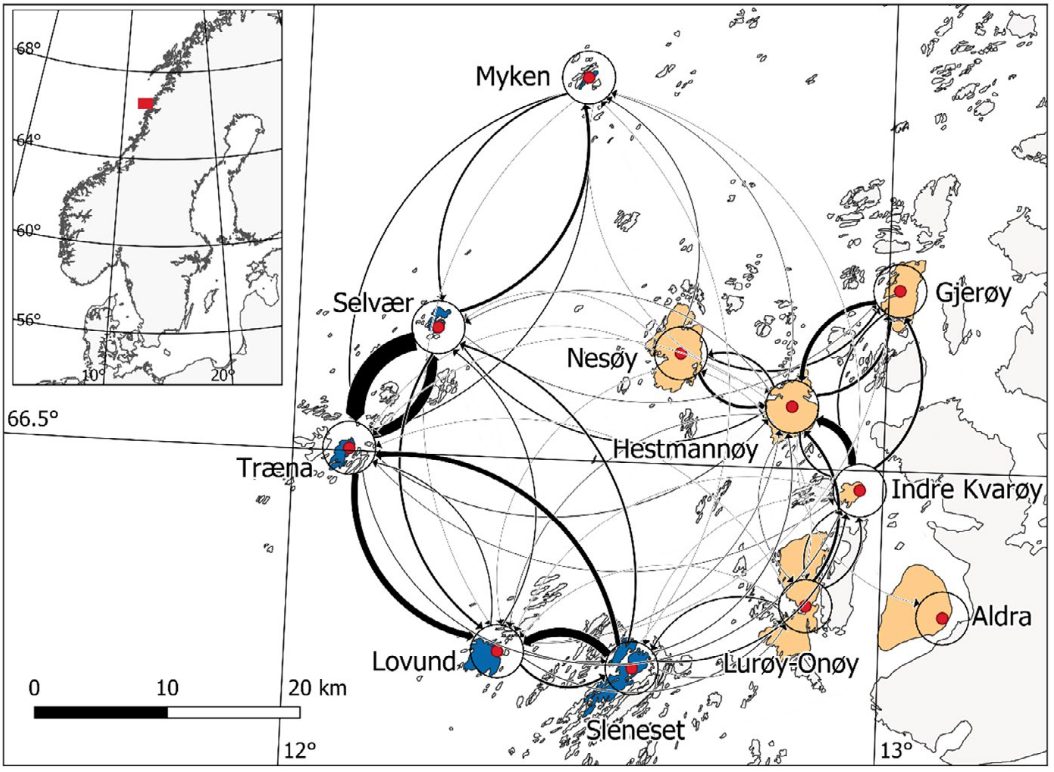
\includegraphics[width=0.8\linewidth]{Figures/Methods/Dispersal (ranke).png}
    \caption[Map of study area]{Map of the study area. Inner islands are in yellow, and outer islands are in blue. The arrows display emigration patterns in the period $1993-2014$. Increased thickness of the arrows indicates a larger volume of emigration (\cite{ranke_spatial_2021}).}
    \label{fig:dispersal on the map}
\end{figure}

The phenotypic and environmental data are found in \texttt{pheno\_env\_F\_ROH\_aligned.rds}, and run configurations can be found in \texttt{26\-01\-27\_run2.R}.

We performed principal component analysis (PCA) in PLINK on the genotype dataset after standard quality-control preprocessing. Specifically, we restricted the analysis to a predefined set of individuals using a keep-file, removed rare variants by applying a minor allele frequency threshold of $MAF \geq 0.01$, filtered SNPs with high missingness (variant call rate filter; $geno \leq 0.10$), and excluded individuals with excessive missing genotypes ($mind \leq 0.05$). PCA was then computed on the filtered dataset, and the first $K$ principal components were exported for downstream analyses.


%% 2) outcome 

The goal of this analysis is to find the $K$ that yields the best predictive accuracy on the observed $0/1$ scale. The AUC is reportet for each fitting, in addition to predicted probabilities, breeding values, variance estimates and heritability estimates. These are used for model assessment later.  


%% 3) PC set (whole datasett and describe the grid 

To limit the number of genetic predictors, we did a PCA on the whole SNP dataset. After PCA the genotype matrix $\mathbf{Z} \in \mathbb{R}^{N \times m}$, where $N = 3422$ individuals and $m = 65 244$ SNPs is reduced to $\mathbf{Z}^\star \in \mathbb{R}{N \times K_{max}}$, where $K_{max} = 1500$. To test the accuracy as a function of the number of PCs $K$ we fit the model several times and increase $K = 100, 200, \dots, 1500$.


%% 4) model fitting 

Using the observed phenotypes, we fitted a Bernoulli GLMM with the BPCRR as the linear predictor. The model specification and estimation procedure are described below.

The phenotypes were modeled using a Bernoulli likelihood with a logit link. For any given individual $i$, the linear predictor on the liability scale was
$$
\mathrm{logit}(p_i) = \eta_i =   \beta_0 + \beta_{sex}x_{sex, i} + \beta_{F} x_{F_ROH, i} + \gamma_{year} w_{year, i} + \gamma_{island} w_{island, i} + \sum_{k=1}^K z_{ik}^\star u_k^\star \quad i = 1, 2, \dots, N \ ,
$$
where $\beta_0$ is the intercept, $\beta_{sex}$ and $\beta_F$ are the fixed effects, $\gamma_{year}$ and $\gamma_{island}$ are the random effects for hatch year and natal island respectively, $z_{ik}^\star$ is the $k$'th PC score for individual $i$, $u_k^\star$ is the corresponding effect, and $K$ is the total number of PCs included in the model. The PCs were computed from the centered SNP matrix using singular value decomposition. All PC effects were assigned the common ridge prior,
$$
u_k^\star \sim N(0, \sigma_{u^\star}^2) \quad k = 1, 2, \dots, K\ ,
$$
with a shared prior variance $\sigma_{u^\star}^2$. This prior variance was chosen based on additive genetic variance estimates done by \textcite{saatoglu_genetic_2024}. 
To obtain a prior on the effects that induce the desired level of additive genetic variance, we scale the prior variance according to the empirical variances of the principal components,
$$
\sigma_{u^\star}^2 = 
\frac{V_A}{\sum_{k=1}^K \mathrm{Var}(\mathbf{z}_k^\star)} \ ,
$$
where $\mathrm{Var}(\mathbf{z}_k^\star)$ is the variance contribution from the $k$'th PC $\mathbf{z}_k^\star$. This prior is chosen to give ridge-type shrinkage on the PC effects (\cite{aspheim_bayesian_2024}).
The intercept $\\beta_0$ was treated as a fixed effect using INLA’s default prior, and posterior means of the PC effects $\hat{u}_k^\star$  were used for prediction. Estimated breeding values were obtained as
%
$$
\hat{a_i} = \sum_{k=1}^K z_{ik}^\star \hat{u}_k^\star \quad i = 1, 2, \dots, N \ ,
$$
%
and predicted probabilities $\hat{p}_i$ were computed by applying the inverse-logit, defined in equation \eqref{eq:inverse-link}, to the linear predictor
%
$$
\hat{p_i} = \frac{e^{\hat{\eta}_i}}{1 + e^{\hat{\eta}_i}} \quad i = 1, 2, \dots, N \ .
$$
These probabilities were used to assess predictive performance under
different choices of the number of principal components.  

%% 5) train test split 

The model was fitted $5$ times with a different stratified train/test split, and the seeds used for splitting is saved in the results folder. This split was used for all $K$ each time to ensure comparable results. 

%% 6) Hyper parameters (fixed VA osv. )



%% 7) Outputs 

For each fit the script returns 
\begin{itemize}
  \item \textbf{Splitt og indekser:} \texttt{IID}, \texttt{train\_ix}, \texttt{test\_ix}

  \item \textbf{Data/prediksjoner:}
  \begin{itemize}
    \item \texttt{y}, \texttt{y\_test}
    \item \texttt{p\_all} (posterior summary av predikert sannsynlighet for alle)
    \item \texttt{p\_test} (posterior summary på test)
  \end{itemize}

  \item \textbf{Genetiske effekter:}
  \begin{itemize}
    \item \texttt{breeding\_values} (mean/sd/kvantiler per individ fra \texttt{IDX\_Z})
    \item \texttt{breeding\_values\_test}
  \end{itemize}

  \item \textbf{Parameter-/komponentestimater:}
  \begin{itemize}
    \item \texttt{intercept} (fra \texttt{fit\$summary.fixed})
    \item \texttt{VA\_hat} + \texttt{VA\_ci} (fra posterior sampling av \texttt{betaPC} og $\mathrm{var}(\texttt{XX} \%*\% \texttt{beta})$)
    \item \texttt{h2\_liability} + \texttt{h2\_ci} (med $V_{\text{logit}} = \pi^2/3$ + varians fra \texttt{hatchYear}/\texttt{NatalIsland})
  \end{itemize}

  \item \textbf{Evalueringsmetrikker:}
  \begin{itemize}
    \item \texttt{auc} (\texttt{pROC} på test)
    \item \texttt{brier} (på test)
  \end{itemize}

  \item \textbf{Fit-mål:}
  \begin{itemize}
    \item \texttt{fit\_summary} med \texttt{dic} og \texttt{waic}
  \end{itemize}
\end{itemize}
